% Options for packages loaded elsewhere
\PassOptionsToPackage{unicode}{hyperref}
\PassOptionsToPackage{hyphens}{url}
%
\documentclass[
]{article}
\usepackage{amsmath,amssymb}
\usepackage{lmodern}
\usepackage{ifxetex,ifluatex}
\ifnum 0\ifxetex 1\fi\ifluatex 1\fi=0 % if pdftex
  \usepackage[T1]{fontenc}
  \usepackage[utf8]{inputenc}
  \usepackage{textcomp} % provide euro and other symbols
\else % if luatex or xetex
  \usepackage{unicode-math}
  \defaultfontfeatures{Scale=MatchLowercase}
  \defaultfontfeatures[\rmfamily]{Ligatures=TeX,Scale=1}
\fi
% Use upquote if available, for straight quotes in verbatim environments
\IfFileExists{upquote.sty}{\usepackage{upquote}}{}
\IfFileExists{microtype.sty}{% use microtype if available
  \usepackage[]{microtype}
  \UseMicrotypeSet[protrusion]{basicmath} % disable protrusion for tt fonts
}{}
\makeatletter
\@ifundefined{KOMAClassName}{% if non-KOMA class
  \IfFileExists{parskip.sty}{%
    \usepackage{parskip}
  }{% else
    \setlength{\parindent}{0pt}
    \setlength{\parskip}{6pt plus 2pt minus 1pt}}
}{% if KOMA class
  \KOMAoptions{parskip=half}}
\makeatother
\usepackage{xcolor}
\IfFileExists{xurl.sty}{\usepackage{xurl}}{} % add URL line breaks if available
\IfFileExists{bookmark.sty}{\usepackage{bookmark}}{\usepackage{hyperref}}
\hypersetup{
  pdftitle={The Gaussian Mixture Copula for Inference with Missing Data},
  pdfauthor={Joe Feldman},
  hidelinks,
  pdfcreator={LaTeX via pandoc}}
\urlstyle{same} % disable monospaced font for URLs
\usepackage[margin=1in]{geometry}
\usepackage{color}
\usepackage{fancyvrb}
\newcommand{\VerbBar}{|}
\newcommand{\VERB}{\Verb[commandchars=\\\{\}]}
\DefineVerbatimEnvironment{Highlighting}{Verbatim}{commandchars=\\\{\}}
% Add ',fontsize=\small' for more characters per line
\usepackage{framed}
\definecolor{shadecolor}{RGB}{248,248,248}
\newenvironment{Shaded}{\begin{snugshade}}{\end{snugshade}}
\newcommand{\AlertTok}[1]{\textcolor[rgb]{0.94,0.16,0.16}{#1}}
\newcommand{\AnnotationTok}[1]{\textcolor[rgb]{0.56,0.35,0.01}{\textbf{\textit{#1}}}}
\newcommand{\AttributeTok}[1]{\textcolor[rgb]{0.77,0.63,0.00}{#1}}
\newcommand{\BaseNTok}[1]{\textcolor[rgb]{0.00,0.00,0.81}{#1}}
\newcommand{\BuiltInTok}[1]{#1}
\newcommand{\CharTok}[1]{\textcolor[rgb]{0.31,0.60,0.02}{#1}}
\newcommand{\CommentTok}[1]{\textcolor[rgb]{0.56,0.35,0.01}{\textit{#1}}}
\newcommand{\CommentVarTok}[1]{\textcolor[rgb]{0.56,0.35,0.01}{\textbf{\textit{#1}}}}
\newcommand{\ConstantTok}[1]{\textcolor[rgb]{0.00,0.00,0.00}{#1}}
\newcommand{\ControlFlowTok}[1]{\textcolor[rgb]{0.13,0.29,0.53}{\textbf{#1}}}
\newcommand{\DataTypeTok}[1]{\textcolor[rgb]{0.13,0.29,0.53}{#1}}
\newcommand{\DecValTok}[1]{\textcolor[rgb]{0.00,0.00,0.81}{#1}}
\newcommand{\DocumentationTok}[1]{\textcolor[rgb]{0.56,0.35,0.01}{\textbf{\textit{#1}}}}
\newcommand{\ErrorTok}[1]{\textcolor[rgb]{0.64,0.00,0.00}{\textbf{#1}}}
\newcommand{\ExtensionTok}[1]{#1}
\newcommand{\FloatTok}[1]{\textcolor[rgb]{0.00,0.00,0.81}{#1}}
\newcommand{\FunctionTok}[1]{\textcolor[rgb]{0.00,0.00,0.00}{#1}}
\newcommand{\ImportTok}[1]{#1}
\newcommand{\InformationTok}[1]{\textcolor[rgb]{0.56,0.35,0.01}{\textbf{\textit{#1}}}}
\newcommand{\KeywordTok}[1]{\textcolor[rgb]{0.13,0.29,0.53}{\textbf{#1}}}
\newcommand{\NormalTok}[1]{#1}
\newcommand{\OperatorTok}[1]{\textcolor[rgb]{0.81,0.36,0.00}{\textbf{#1}}}
\newcommand{\OtherTok}[1]{\textcolor[rgb]{0.56,0.35,0.01}{#1}}
\newcommand{\PreprocessorTok}[1]{\textcolor[rgb]{0.56,0.35,0.01}{\textit{#1}}}
\newcommand{\RegionMarkerTok}[1]{#1}
\newcommand{\SpecialCharTok}[1]{\textcolor[rgb]{0.00,0.00,0.00}{#1}}
\newcommand{\SpecialStringTok}[1]{\textcolor[rgb]{0.31,0.60,0.02}{#1}}
\newcommand{\StringTok}[1]{\textcolor[rgb]{0.31,0.60,0.02}{#1}}
\newcommand{\VariableTok}[1]{\textcolor[rgb]{0.00,0.00,0.00}{#1}}
\newcommand{\VerbatimStringTok}[1]{\textcolor[rgb]{0.31,0.60,0.02}{#1}}
\newcommand{\WarningTok}[1]{\textcolor[rgb]{0.56,0.35,0.01}{\textbf{\textit{#1}}}}
\usepackage{graphicx}
\makeatletter
\def\maxwidth{\ifdim\Gin@nat@width>\linewidth\linewidth\else\Gin@nat@width\fi}
\def\maxheight{\ifdim\Gin@nat@height>\textheight\textheight\else\Gin@nat@height\fi}
\makeatother
% Scale images if necessary, so that they will not overflow the page
% margins by default, and it is still possible to overwrite the defaults
% using explicit options in \includegraphics[width, height, ...]{}
\setkeys{Gin}{width=\maxwidth,height=\maxheight,keepaspectratio}
% Set default figure placement to htbp
\makeatletter
\def\fps@figure{htbp}
\makeatother
\setlength{\emergencystretch}{3em} % prevent overfull lines
\providecommand{\tightlist}{%
  \setlength{\itemsep}{0pt}\setlength{\parskip}{0pt}}
\setcounter{secnumdepth}{-\maxdimen} % remove section numbering
\ifluatex
  \usepackage{selnolig}  % disable illegal ligatures
\fi

\title{The Gaussian Mixture Copula for Inference with Missing Data}
\author{Joe Feldman}
\date{7/10/2022}

\begin{document}
\maketitle

\hypertarget{installation}{%
\section{Installation}\label{installation}}

\begin{Shaded}
\begin{Highlighting}[]
\CommentTok{\# library(devtools)}
\CommentTok{\# remotes::install\_github(\textquotesingle{}jfeldman396/GMCImpute\textquotesingle{})}

\FunctionTok{library}\NormalTok{(GMCImpute)}
\end{Highlighting}
\end{Shaded}

\hypertarget{background-missing-data}{%
\section{Background: Missing Data}\label{background-missing-data}}

Missing data is commonplace in survey and fused data sets, necessitating
sophisticated methods for dealing with missingness when deriving
inference. First, these data sets may be comprised of mixed data types,
such as continuous, count, and nominal variables. Second, the missing
data may bias certain properties of the data set. As a result, a
complete case analysis, where the analyst drops any observations with
missing values, would lead to misleading insights on the data.

Consider the following simulated example of a continuous variable
\(X_{1}\), a count variable \(X_{2}\), and a binary variable \(X_{3}\),
where missing values in \(X_{2}\) and \(X_{3}\) are correlated to large
values of \(X_{1}\) in absolute value.

\begin{Shaded}
\begin{Highlighting}[]
\NormalTok{num}\OtherTok{=} \DecValTok{500}
\NormalTok{X1}\OtherTok{\textless{}{-}}\FunctionTok{rnorm}\NormalTok{(num)}
\NormalTok{X2}\OtherTok{\textless{}{-}} \FunctionTok{rpois}\NormalTok{(num,}\DecValTok{5}\SpecialCharTok{*}\FunctionTok{abs}\NormalTok{(X1))}
\NormalTok{X3}\OtherTok{\textless{}{-}} \FunctionTok{as.factor}\NormalTok{(}\FunctionTok{rbernoulli}\NormalTok{(num,}\FunctionTok{pnorm}\NormalTok{(}\SpecialCharTok{{-}}\NormalTok{.}\DecValTok{5}\SpecialCharTok{+}\FunctionTok{scale}\NormalTok{(X2))))}
\NormalTok{X}\OtherTok{\textless{}{-}} \FunctionTok{data.frame}\NormalTok{(X1,X2,X3)}

\NormalTok{R }\OtherTok{=} \FunctionTok{t}\NormalTok{(}\FunctionTok{sapply}\NormalTok{(}\DecValTok{1}\SpecialCharTok{:}\NormalTok{num, }\ControlFlowTok{function}\NormalTok{(x)}\FunctionTok{rbernoulli}\NormalTok{(}\DecValTok{2}\NormalTok{, }\AttributeTok{p =} \FunctionTok{pnorm}\NormalTok{(}\SpecialCharTok{{-}}\NormalTok{.}\DecValTok{5} \SpecialCharTok{+}\NormalTok{ .}\DecValTok{5}\SpecialCharTok{*}\FunctionTok{abs}\NormalTok{(X1[x]))))) }\CommentTok{\# missingness mechanism}
\NormalTok{X\_noMis }\OtherTok{=}\NormalTok{ X}
\NormalTok{X[}\FunctionTok{which}\NormalTok{(R[,}\DecValTok{1}\NormalTok{] }\SpecialCharTok{==}\NormalTok{ T),}\DecValTok{2}\NormalTok{] }\OtherTok{=} \ConstantTok{NA}
\NormalTok{X[}\FunctionTok{which}\NormalTok{(R[,}\DecValTok{2}\NormalTok{] }\SpecialCharTok{==}\NormalTok{ T),}\DecValTok{3}\NormalTok{] }\OtherTok{=} \ConstantTok{NA}
\end{Highlighting}
\end{Shaded}

We can visualize bias that the mechanism creates in \(X_{2}, X_{3}\)
with the following plots.

\begin{verbatim}
## Warning: Removed 227 rows containing missing values (geom_point).
\end{verbatim}

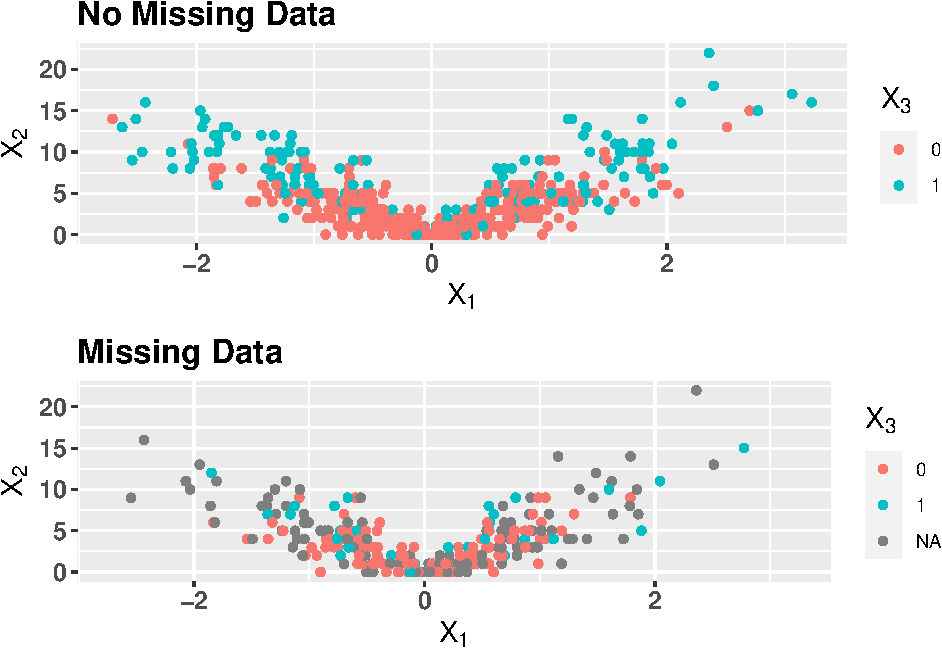
\includegraphics{README_files/figure-latex/unnamed-chunk-2-1.pdf}

As you can see, both margins are affected. We show a comparison of the
empirical cdfs of \(X_{2}\) before and after inputting missing values,
while the incidence of positive indicators is greatly reduced for
\(X_{3}\)

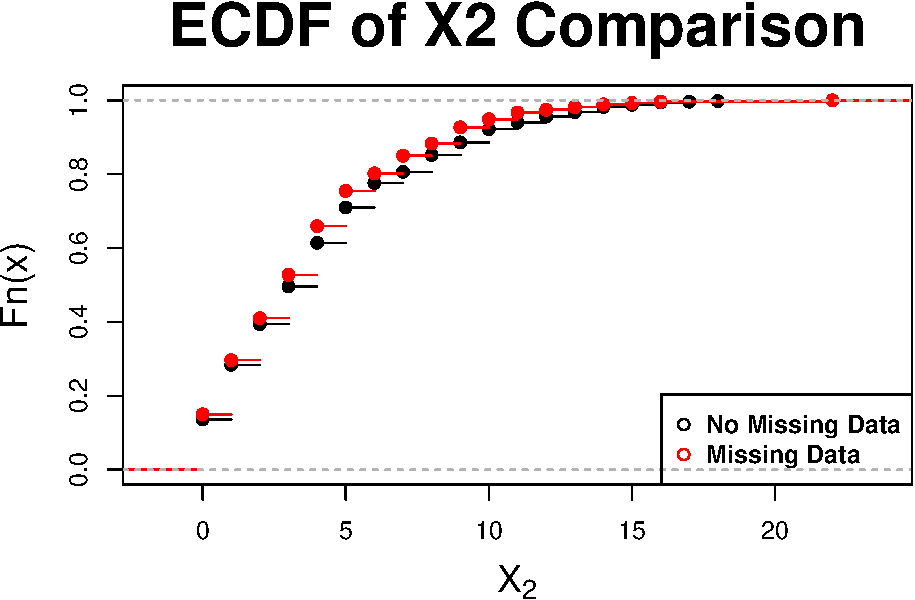
\includegraphics{README_files/figure-latex/unnamed-chunk-3-1.pdf}

\hypertarget{the-gaussian-mixture-copula-with-margin-adjustment}{%
\section{The Gaussian Mixture Copula with Margin
Adjustment}\label{the-gaussian-mixture-copula-with-margin-adjustment}}

The function \texttt{GMC\_Impute} allows users to fit a Gaussian mixture
copula to data comprised of unordered categorical, binary, count and
continuous data types with missing values. This is done through
utilization of the extended rank-probit likelihood, which enables copula
estimation on the aforementioned data types. The function then produces
a user specified number of multiple imputations.

The model is given by
\[z_{i} \sim N(\Lambda \eta_{i}, \Sigma),\ \eta_{i} \sim \sum_{h=1}^{H^{*}\leq H} \pi_{h}N(\mu_{h},\Delta_{h})\\
\Sigma \sim Gamma(a_{\sigma},b_{\sigma}),\lambda_{jh} \sim N(0, \phi_{jh}^{-1}\tau_{h}^{-1})\\
\phi_{jh} \sim Gamma(\nu/2,\nu/2), \tau_{h} = \prod_{l=1}^{h}\delta_{h}^{\tau} \\
\text{with} \ \delta^{\tau}_{1} \sim Gamma(a_{1},1) \ \text{and} \ \delta^{\tau}_{l} \sim Gamma(a_{2},1), \ l\geq 2, \ a_{2} \geq 1\]

For the mixing weights, we use the truncated dirichlet process prior,
which specifies an upper bound for the number of clusters and allows the
data to inform which \(H^{*}\) get populated

\[\pi_{h} = V_{h}\prod_{l<h} (1-V_{l}),\  V_{h}\sim Beta(1, \alpha_{\pi})\\
        \alpha_{\pi} \sim Gamma(a_{\alpha}, b_{\alpha})\]

For the prior on \(\eta\), we use a Normal-Inverse Wishart:
\((\boldsymbol{\mu_{h}, \Delta_{h}}) \sim Normal-InverseWishart(\boldsymbol{\mu_{0}}, \delta^{2}*\boldsymbol{I_{k}},\kappa_{0}, \nu_{mix})\)

Key to gaussian mixture copula are the marginal distributions of each
variable in the data, as latent variables, modeled with finite mixture
are linked to the observed scale using the inverse marginal distribution
function. Previous work estimates these margins empirically, which is
problematic given that the missing data clearly biases these estimates.
The margin adjustment corrects these biases, yielding proper inference
with missing data.

\hypertarget{fitting-the-model}{%
\section{Fitting the model}\label{fitting-the-model}}

To use the function, the user can specify a number of properties of the
model:

\begin{itemize}
\tightlist
\item
  \texttt{nImp}: The number of imputations to create
\item
  \texttt{H}: The upper bound for the number of clusters in the
  truncated DP mixture
\item
  \texttt{k.star}: The dimension of the latent factors, defult is
  \texttt{ceiling(0.7*p)}
\item
  \texttt{nsamp}: number of interations in the MCMC
\item
  \texttt{burn}: burn-in before posterior samples are saved
\item
  \texttt{hyperparams}:

  \begin{itemize}
  \tightlist
  \item
    \texttt{delta}: to the precision of the prior covariance. This
    parameter has been the most influential in the discovery of new
    clusters. Lower to find more clusters. Default value is 10
  \item
    \texttt{k.star}: change to increase or decrease dimension of latent
    factors
  \item
    \texttt{a\_alpha}
  \item
    \texttt{b\_alpha}
  \item
    \texttt{nu\_mix}
  \item
    \texttt{kappa\_0}
  \item
    \texttt{nu}
  \item
    \texttt{a1}
  \item
    \texttt{a2}
  \item
    \texttt{a.sigma}
  \item
    \texttt{b.sigma}
  \item
    \texttt{D\_0}: k.star dimensional identity
  \end{itemize}
\end{itemize}

Default values are included in the function documentation, but we
recommend altering \(\delta\) to improve model fit. The function is
called below:

\begin{Shaded}
\begin{Highlighting}[]
\NormalTok{hyperparams }\OtherTok{=} \FunctionTok{list}\NormalTok{(}\AttributeTok{delta =} \DecValTok{10}\NormalTok{,}
                   \AttributeTok{k.star =} \DecValTok{2}\NormalTok{,}
                   \AttributeTok{plugin.threshold =} \DecValTok{100}\NormalTok{,}
                   \AttributeTok{a\_alpha =} \DecValTok{1}\NormalTok{,}
                   \AttributeTok{b\_alpha =} \DecValTok{3}\NormalTok{,}
                   \AttributeTok{nu\_mix =} \DecValTok{4}\NormalTok{,}
                   \AttributeTok{kappa\_0 =}\NormalTok{ .}\DecValTok{001}\NormalTok{,}
                   \AttributeTok{nu =} \DecValTok{3}\NormalTok{,}
                   \AttributeTok{a1 =} \DecValTok{2}\NormalTok{,}
                   \AttributeTok{a2 =} \DecValTok{3}\NormalTok{,}
                   \AttributeTok{a.sigma =} \DecValTok{1}\NormalTok{,}
                   \AttributeTok{b.sigma =}\NormalTok{ .}\DecValTok{3}\NormalTok{,}
                   \AttributeTok{D\_0 =} \FunctionTok{diag}\NormalTok{(}\DecValTok{1}\NormalTok{,}\DecValTok{2}\NormalTok{))}
\NormalTok{imps}\OtherTok{\textless{}{-}}\FunctionTok{GMC\_Impute}\NormalTok{(}\AttributeTok{Data =}\NormalTok{ X, }\AttributeTok{nImp =} \DecValTok{5}\NormalTok{,}\AttributeTok{hyperparams =}\NormalTok{ hyperparams, }\AttributeTok{burn =} \DecValTok{5000}\NormalTok{,}\AttributeTok{nsamp =} \DecValTok{10000}\NormalTok{, }\AttributeTok{seed =} \DecValTok{47}\NormalTok{)}
\end{Highlighting}
\end{Shaded}

\texttt{GMC\_Impute} returns \texttt{nImp} imputations, as well as
posterior samples of Copula parameters which may be used for simulation
of posterior predictive data sets or posterior inference. See
documentation for format.

\hypertarget{plotting-results}{%
\section{Plotting Results}\label{plotting-results}}

\hypertarget{visualizing-imputations}{%
\subsection{Visualizing Imputations:}\label{visualizing-imputations}}

\begin{verbatim}
## Warning: Removed 1 rows containing missing values (geom_point).
\end{verbatim}

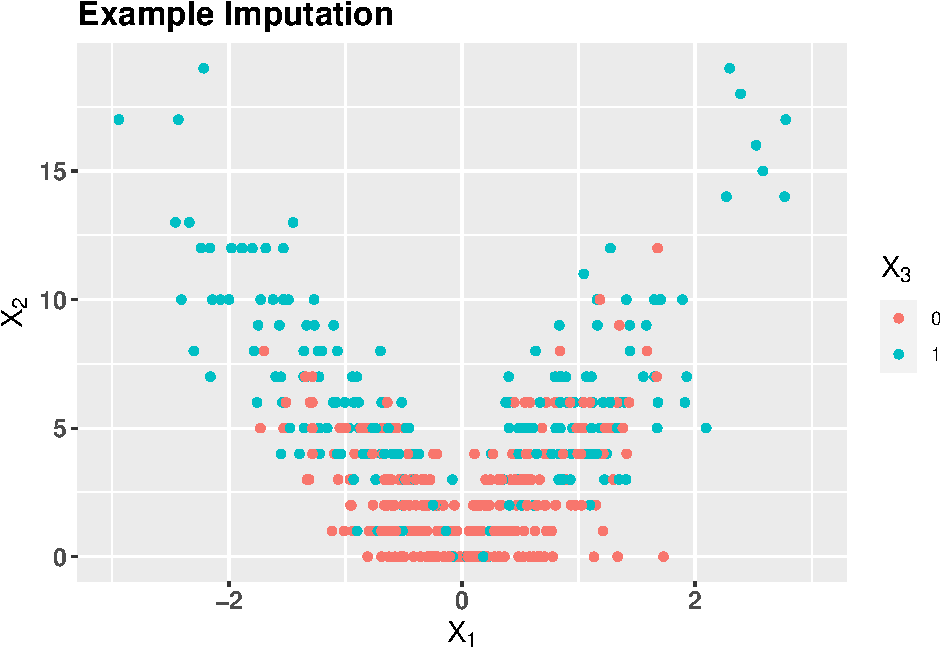
\includegraphics{README_files/figure-latex/unnamed-chunk-4-1.pdf}

\hypertarget{plotting-posterior-samples-from-the-margin-adjustment}{%
\subsection{Plotting posterior samples from the margin
adjustment}\label{plotting-posterior-samples-from-the-margin-adjustment}}

We can plot posterior samples of the marginal distribution of \(X_{2}\),
as well as point-wise posterior means:

\begin{Shaded}
\begin{Highlighting}[]
  \FunctionTok{par}\NormalTok{(}\AttributeTok{mar =} \FunctionTok{c}\NormalTok{(}\DecValTok{5}\NormalTok{,}\DecValTok{6}\NormalTok{,}\DecValTok{4}\NormalTok{,}\DecValTok{2}\NormalTok{))}
\NormalTok{range }\OtherTok{=} \FunctionTok{range}\NormalTok{(imps}\SpecialCharTok{$}\NormalTok{Support[[}\DecValTok{3}\NormalTok{]][}\DecValTok{1}\NormalTok{,}\DecValTok{2}\SpecialCharTok{:}\DecValTok{18}\NormalTok{]) }\CommentTok{\# get support}
\NormalTok{quantiles }\OtherTok{=}\NormalTok{ imps}\SpecialCharTok{$}\NormalTok{Quantiles[[}\DecValTok{3}\NormalTok{]] }\CommentTok{\#get quantiles}
 \FunctionTok{plot}\NormalTok{(range[}\DecValTok{1}\NormalTok{]}\SpecialCharTok{:}\NormalTok{range[}\DecValTok{2}\NormalTok{],quantiles[}\DecValTok{1}\NormalTok{,}\DecValTok{2}\SpecialCharTok{:}\NormalTok{(range[}\DecValTok{2}\NormalTok{]}\SpecialCharTok{+}\DecValTok{2}\NormalTok{)],}
      \AttributeTok{col =} \StringTok{"gray"}\NormalTok{,}
      \AttributeTok{type =} \StringTok{\textquotesingle{}b\textquotesingle{}}\NormalTok{,}
       \AttributeTok{xlab =} \FunctionTok{expression}\NormalTok{(X[}\DecValTok{2}\NormalTok{]),}
       \AttributeTok{ylab =} \FunctionTok{expression}\NormalTok{(}\FunctionTok{P}\NormalTok{(X[}\DecValTok{2}\NormalTok{] }\SpecialCharTok{\textless{}=}\NormalTok{ x)),}
       \AttributeTok{main =} \StringTok{"Posterior Samples of F\_X2"}\NormalTok{,}
       \AttributeTok{cex.lab =} \FloatTok{1.5}\NormalTok{,}
       \AttributeTok{cex.main =} \DecValTok{2}\NormalTok{)}
  \FunctionTok{sapply}\NormalTok{(}\DecValTok{2}\SpecialCharTok{:}\DecValTok{5000}\NormalTok{,}\ControlFlowTok{function}\NormalTok{(x)}\FunctionTok{points}\NormalTok{(range[}\DecValTok{1}\NormalTok{]}\SpecialCharTok{:}\NormalTok{range[}\DecValTok{2}\NormalTok{],quantiles[x,}\DecValTok{2}\SpecialCharTok{:}\NormalTok{(range[}\DecValTok{2}\NormalTok{]}\SpecialCharTok{+}\DecValTok{2}\NormalTok{)], }\AttributeTok{col =}\StringTok{\textquotesingle{}gray\textquotesingle{}}\NormalTok{, }\AttributeTok{type =} \StringTok{\textquotesingle{}b\textquotesingle{}}\NormalTok{))}
  \FunctionTok{lines}\NormalTok{(}\FunctionTok{ecdf}\NormalTok{(X\_noMis}\SpecialCharTok{$}\NormalTok{X2), }\AttributeTok{cex =} \DecValTok{2}\NormalTok{)}
  \FunctionTok{points}\NormalTok{(range[}\DecValTok{1}\NormalTok{]}\SpecialCharTok{:}\NormalTok{range[}\DecValTok{2}\NormalTok{],}\FunctionTok{colMeans}\NormalTok{(quantiles[}\DecValTok{2}\SpecialCharTok{:}\DecValTok{5000}\NormalTok{,}\DecValTok{2}\SpecialCharTok{:}\NormalTok{(range[}\DecValTok{2}\NormalTok{]}\SpecialCharTok{+}\DecValTok{2}\NormalTok{)]),}\AttributeTok{pch =}\DecValTok{2}\NormalTok{, }\AttributeTok{cex =} \DecValTok{2}\NormalTok{)}
  \FunctionTok{lines}\NormalTok{(}\FunctionTok{ecdf}\NormalTok{(X}\SpecialCharTok{$}\NormalTok{X2), }\AttributeTok{col =} \DecValTok{2}\NormalTok{, }\AttributeTok{cex =} \DecValTok{2}\NormalTok{)}
    \FunctionTok{legend}\NormalTok{(}\StringTok{"bottomright"}\NormalTok{,}\FunctionTok{c}\NormalTok{(}\StringTok{"ECDF w/o Mis"}\NormalTok{,}\StringTok{"ECDF w/ Mis"}\NormalTok{,}\StringTok{"Posterior Mean"}\NormalTok{), }\AttributeTok{pch =} \FunctionTok{c}\NormalTok{(}\DecValTok{16}\NormalTok{,}\DecValTok{16}\NormalTok{,}\DecValTok{2}\NormalTok{),}\AttributeTok{col =} \FunctionTok{c}\NormalTok{(}\DecValTok{1}\NormalTok{,}\DecValTok{2}\NormalTok{,}\DecValTok{1}\NormalTok{),}\AttributeTok{bty =} \StringTok{\textquotesingle{}n\textquotesingle{}}\NormalTok{, }\AttributeTok{cex =} \FloatTok{1.3}\NormalTok{, }\AttributeTok{text.font =} \DecValTok{2}\NormalTok{)}
\end{Highlighting}
\end{Shaded}

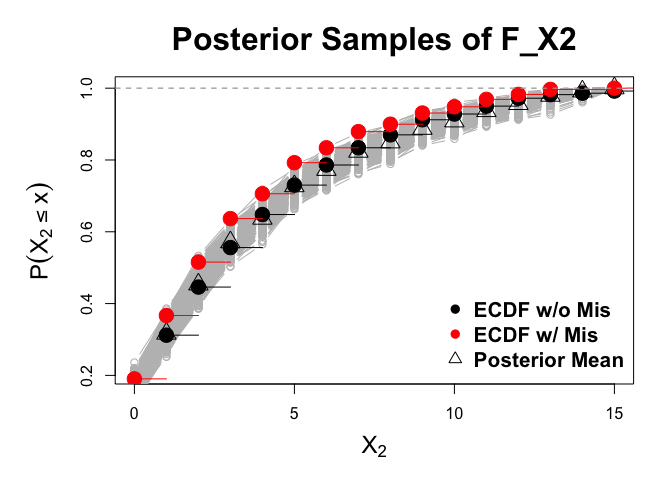
\includegraphics{README_files/figure-latex/unnamed-chunk-5-1.pdf}

\hypertarget{simulating-predictive-data-sets}{%
\section{Simulating Predictive Data
Sets}\label{simulating-predictive-data-sets}}

Finally, we can use the posterior samples to generative posterior
predictive data sets for checks and inference. This is done by using the
returned samples from GMC\_Impute

\begin{Shaded}
\begin{Highlighting}[]
\CommentTok{\#use the 2000th sample as an example}

\CommentTok{\#GMC parameters}
\NormalTok{mu }\OtherTok{=} \FunctionTok{lapply}\NormalTok{(}\DecValTok{1}\SpecialCharTok{:}\DecValTok{25}\NormalTok{, }\ControlFlowTok{function}\NormalTok{(x) }\FunctionTok{return}\NormalTok{(imps}\SpecialCharTok{$}\NormalTok{mus[[x]][}\DecValTok{2000}\NormalTok{,]))}
\NormalTok{alpha }\OtherTok{=} \FunctionTok{rep}\NormalTok{(}\DecValTok{0}\NormalTok{,}\DecValTok{3}\NormalTok{)}
\NormalTok{Delta }\OtherTok{=} \FunctionTok{lapply}\NormalTok{(}\DecValTok{1}\SpecialCharTok{:}\DecValTok{25}\NormalTok{, }\ControlFlowTok{function}\NormalTok{(x) }\FunctionTok{return}\NormalTok{(imps}\SpecialCharTok{$}\NormalTok{Deltas[[x]][}\DecValTok{2000}\NormalTok{,,]))}
\NormalTok{Lambda }\OtherTok{=}\NormalTok{ imps}\SpecialCharTok{$}\NormalTok{Lambdas[}\DecValTok{2000}\NormalTok{,,]}
\NormalTok{pi\_h }\OtherTok{=}\NormalTok{ imps}\SpecialCharTok{$}\NormalTok{pis[}\DecValTok{2000}\NormalTok{,]}
\NormalTok{Sigma.diag}\OtherTok{=}\NormalTok{ imps}\SpecialCharTok{$}\NormalTok{Sigmas[}\DecValTok{2000}\NormalTok{,]}
\CommentTok{\#column names and memberships}
\NormalTok{col\_mem }\OtherTok{=}\NormalTok{ imps}\SpecialCharTok{$}\NormalTok{col\_mem}
\NormalTok{cat\_col\_names }\OtherTok{=}\NormalTok{ imps}\SpecialCharTok{$}\NormalTok{cat\_col\_names}
\NormalTok{bin\_col\_names }\OtherTok{=}\NormalTok{ imps}\SpecialCharTok{$}\NormalTok{bin\_col\_names}
\NormalTok{count\_col\_names }\OtherTok{=}\NormalTok{ imps}\SpecialCharTok{$}\NormalTok{count\_col\_names}
\NormalTok{cont\_col\_names }\OtherTok{=}\NormalTok{ imps}\SpecialCharTok{$}\NormalTok{con\_col\_names}
\NormalTok{H }\OtherTok{=} \DecValTok{25}
\NormalTok{Y }\OtherTok{=}\NormalTok{ imps}\SpecialCharTok{$}\NormalTok{dat}
\NormalTok{z }\OtherTok{=}\NormalTok{ imps}\SpecialCharTok{$}\NormalTok{zs[}\DecValTok{2000}\NormalTok{,]}
\NormalTok{Fns }\OtherTok{=} \FunctionTok{vector}\NormalTok{(}\StringTok{\textquotesingle{}list\textquotesingle{}}\NormalTok{, }\DecValTok{3}\NormalTok{) }\CommentTok{\#format marginal distributions}
\ControlFlowTok{for}\NormalTok{(i }\ControlFlowTok{in} \DecValTok{1}\SpecialCharTok{:}\DecValTok{3}\NormalTok{)\{}
\NormalTok{  support }\OtherTok{=}\NormalTok{ imps}\SpecialCharTok{$}\NormalTok{Support[[i]][}\DecValTok{2000}\NormalTok{,]}
\NormalTok{  qs }\OtherTok{=}\NormalTok{ imps}\SpecialCharTok{$}\NormalTok{Quantiles[[i]][}\DecValTok{2000}\NormalTok{,]}
\NormalTok{  Fj }\OtherTok{=} \FunctionTok{cbind}\NormalTok{(support,}\FunctionTok{rep}\NormalTok{(}\DecValTok{0}\NormalTok{,}\FunctionTok{length}\NormalTok{(support)),qs)}
\NormalTok{  Fns[[i]] }\OtherTok{=}\NormalTok{ Fj}
  
\NormalTok{\}}

\NormalTok{Y }\OtherTok{=}\NormalTok{ imps}\SpecialCharTok{$}\NormalTok{dat }\CommentTok{\#for }
\NormalTok{H }\OtherTok{=}\DecValTok{25}

\NormalTok{pred}\OtherTok{\textless{}{-}} \FunctionTok{get\_predictive\_Y}\NormalTok{(}\AttributeTok{n =} \FunctionTok{dim}\NormalTok{(Y)[}\DecValTok{1}\NormalTok{],}
                          \AttributeTok{Lambda =}\NormalTok{ Lambda,}
                          \AttributeTok{mu =}\NormalTok{ mu,}
                          \AttributeTok{alpha =}\NormalTok{ alpha,}
                          \AttributeTok{Delta =}\NormalTok{ Delta,}
                          \AttributeTok{pi\_h =}\NormalTok{ pi\_h,}
                          \AttributeTok{Sigma.diag =}\NormalTok{ Sigma.diag,}
                          \AttributeTok{col\_mem =}\NormalTok{ col\_mem,}
                          \AttributeTok{cat\_col\_names =}\NormalTok{ cat\_col\_names,}
                          \AttributeTok{bin\_col\_names =}\NormalTok{ bin\_col\_names, }
                          \AttributeTok{count\_col\_names =}\NormalTok{ count\_col\_names,}
                          \AttributeTok{cont\_col\_names =}\NormalTok{ cont\_col\_names,}
                          \AttributeTok{H =}\NormalTok{ H,}
                          \AttributeTok{Y =}\NormalTok{ Y,}
                          \AttributeTok{z =}\NormalTok{ z,}
                          \AttributeTok{Fns =}\NormalTok{ Fns,}
                          \AttributeTok{seed =} \DecValTok{2}\NormalTok{)}
\end{Highlighting}
\end{Shaded}

\includegraphics[width=17.44in]{Screen Shot 2022-07-10 at 1.29.59 PM}

\end{document}
